\chapter{Praktische Umsetzung}

\section{Gehäuse}
\label{sec:orge6f5aa8}
Das Gehäuse muss so dimensioniert sein, dass es Eurorack-kompatible Module beherbergen kann. Wichtig ist dabei vor allem der vertikale Abstand der Schienen, auf welchen die Module befestigt werden. Dieser misst laut dem \emph{Doepfer System A100 Handbuch} \cite{doepfer:A-100} 3 \acp{HE}. 1 \ac{HE} beträgt dabei \SI{44.45}{\milli\meter}. Die Breite der Module beträgt ein Vielfaches von \SI{5.08}{\milli\meter}, beziehungsweise 0.2 Zoll. Manche Gehäuse, wie beispielsweise die von der Firma Intellijel können auch Module beherrbergen, die nur eine Höheneinheit hoch sind.

\section{Spannungsquelle}
\label{sec:org502799b}
Eurorack-Synthesizer arbeiten mit Spannungen von \SI{24}{\volt} peak to peak, benötigen also eine Spannungsquelle, welche \SI{-12}{\volt} bis \SI{+12}{\volt} bereitstellen kann. Manche Module benötigen außerdem eine separate \SI{5}{\volt} Leitung, um zum Beispiel Microcontroller zu betreiben. Eine beliebte Wahl in der DIY-Szene ist die Mean Well RT65B PSU, da sie sowohl \SI{\pm 12}{\volt} als auch \SI{5}{\volt} mit einer Stromstärke/Leistung bereitstellt, welche ausreicht um ein Anfängersystem zu versorgen und verhältnismäßig günstig ist \cite{modularsynthlab:rt65b}.

\section{Spannungsverteilung}
\label{sec:org9ef922c}
Die Module werden über ein 10 Pin IDC-Flachbandkabel mit Strom versorgt. Dabei sind die mittleren 6 Pins durchverbunden und geerdet. Die äußeren vier Pins sind paarweise verbunden und liefern jeweils \SI{+12}{\volt} und \SI{-12}{\volt}. Der PIN, welcher auf \SI{-12}{\volt} liegt, ist üblicherweise rot gekennzeichnet.

\section{Transistoren abgleichen}
\label{sec:org14681f5}
Manchmal werden Transistoren benötigt, welche einen möglichst gleichen internen Verstärkungsfaktor besitzen. Bereits aufeinander abgestimmte Transistorpaare sind zwar im Handel erhältlich, jedoch ist es einfach, das Abgleichen von Transistoren selbst vorzunehmen. Baut man den zu messenden Transistor in Schaltkreis \ref{fig:schematic_match} ein, und legt bei \(V_{CC}\) eine Spannung an, kann man seinen internen Verstärkungsfaktor herausfinden, indem man das Potential zwischen Punkt A (beim Kollektor des Transistors) und der Masse misst \cite{match_transistors}:

\begin{figure}
\centering
\begin{circuitikz}[european]
\draw{
(0,0) -- ++(3,0) node[ground]{}
(0,0) to[R, l=\SI{22}{\kilo\ohm}] ++(0,2.5) coordinate (T) to[R, l=\SI{220}{\kilo\ohm}] ++(0,2.5) -- ++(3,0) node[vcc]{$V_{CC}$} coordinate (U)
(T) -- ++(2,0) node[npn, tr circle](Q){}
(Q.C) to[R, l_=\SI{10}{\kilo\ohm}] (Q.C|-U)
(Q.E) to[R, l=\SI{1}{\kilo\ohm}] (Q.E|-0,0)
(Q.C) node[right] {A}
};
\end{circuitikz}
\caption{Schaltkreis zum Abgleichen des internen Verstärkungsfaktors von Transistoren \label{fig:schematic_match}}
\end{figure}

Diese Transistorenpaare sollten auf der Platine in unmittelbarer Nähe zueinander sein, da auch die Temperatur einen Einfluss auf die Eigenschaften eines Transistors hat.

\section{Vactrols}
\label{sec:orge7be7f2}
Ein Vactrol, auf Deutsch oft Optokoppler, ist ein simpler, jedoch etwas ungenauer, spannungskontrollierbarer Widerstand, welcher aus einer Leuchtdiode und einem Lichtabhängigen Wiederstand (\acsu{LDR}) besteht \cite{vactrol}. Er kann benutzt werden, um als variable Widerstände geschaltene Potentiometer zu ersetzen und somit den zugehörigen Parameter spannungskontrollierbar zu machen. Der am Vactrol entstehende Widerstand ist näherungsweise invers proportional zur angelegten Spannung.

Während bereits gefertigte Vactrols im Handel erhältlich sind, ist es vor allem in DIY Kreisen üblich, sie selbst herzustellen. Dabei wird eine \ac{LED}, gemeinsam mit einem \ac{LDR} auf eine Art und Weise in ein lichtundurchlässiges Gehäuse (beispielsweise ein Schrumpfschlauch) gebaut, dass der \ac{LDR} von der \ac{LED} beleuchtet wird. 

\section{Module}
\label{sec:org6f0a43a}

Im Folgenden werden die Module, welche den Synthesizer ausmachen, beschrieben. Jedes dieser Module besteht aus einem Panel, das als User Interface dient, und einer Platine, welche mit den elektronischen Komponenten bestückt ist. Panels besitzen mindestens eine Audiobuchse um \ac{CV}, Audio, Triggersignale und andere Arten von Spannungssignalen auszugeben, eine beliebige Anzahl an Audioeingängen für Kontrollspannungen, Audio-Inputs und ähnlichem und weitere Interfacekomponenten wie beispielsweise Potentiometer, Schalter, Knöpfe und \acp{LED}.

Es gibt verschiedene Möglichkeiten, die elektronischen Komponenten zu verlöten. Beispiele dafür sind:
\begin{itemize}
\item Breadboards:
vor allem geeignet zum Erstellen von Prototypen
\item \ac{THT} Platinen:
eine schnelle Methode, um eine einzelne Platine zu fertigen
\item Selbst geätzte oder vorgefertigte Platinen:
eine Methode mit relativ geringem Fehlerpotential; ideal wenn eine größere Anzahl gleichartiger Platinen gefertigt werden soll, beispielsweise für DIY-Kits
\item "`Deadbug"' Methode:
Eletronische Komponenten werden ohne Platine "`point to point"' miteinander verlötet; resultiert meist in Spaghettiähnlichen Strukturen, bei gekonnter Ausführung können jedoch sehr ästhetische Schaltkreise entstehen.
\end{itemize}

Die elektronischen Komponenten unserer Module sind auf \ac{THT} Platinen gelötet. Diese Platine wird im rechten Winkel in der Mitte des Panels befestigt. Interface-Komponenten, welche vom Benutzerpanel aus zugänglich sein sollen, werden über längere Kabel und Schraubklemmen auf der Platine verbunden.

Als Material für Panels sind Bleche, dünne Holz- oder Plastikplatten oder ähnliches geeignet. Zu bedenken ist dabei:

\begin{itemize}
\item Dicke des Materials:
Zum Bestücken sollte eine bestimmte Dicke nicht überschritten werden (abhängig von den gewählten Potentiometern, Audiobuchsen, Schaltern und Knöpfen)
\item Bearbeitbarkeit:
Es müssen Löcher für Interfacekomponenten gebohrt oder gestanzt werden, und das Material muss zugeschnitten werden
\item Beschriftbarkeit:
Für einfachere Zugänglichkeit und für bessere Ästhetik sollten die Panels bemalt und beschriftet werden
\end{itemize}

Wir benutzen eine dünne, schwarz lackierte Holzplatte als Material für unsere Panels. Diese werden mit transparenter Folie beklebt, welche mit weißem Permanentmarker beschriftet werden kann.
\subsection{Oszillator x2 \label{Osci}}
\label{sec:org9aaa221}
Dieses Modul ist ein simples signalerzeugendes Modul, welches zwei voneinander unabhängige Rechteckswellen im hörbaren Bereich generiert.

\subsubsection{Spezifikationen}
\label{sec:org9644746}
Oszillator 1:
\begin{itemize}
\item Spannung: bis zu \SI{\pm10}{\volt}
\item Frequenzbereich: \SI{40}{\hertz} bis \(\approx\)\SI{2000}{\hertz}
\end{itemize}

Oszillator 2:
\begin{itemize}
\item Spannung: bis zu \SI{\pm10}{\volt}
\item Frequenzbereich: \SI{25}{\hertz} bis \(\approx\)\SI{2000}{\hertz}
\end{itemize}

\subsubsection{Elektronik}
\label{sec:org79578ed}
Als Grundlage dient ein einfacher "`Resistor-Capacitor"' Schwingkreis, welcher einen Schmitt-Trigger nutzt. Das resultierende Signal wird durch einen Spannungsfolger gepuffert, da sonst die Oszillation zusammenbricht. Danach wird das Signal AC gekoppelt, um das positive Offset der Oszillation zu entfernen und ein weiteres Mal gepuffert. Darauf folgt ein einfacher variabler Spannungsteiler als Dämpfungsglied, um die Amplitude regulieren zu können. \ref{fig:schematic_oscillator}

\subsubsection{Benutzung}
\label{sec:org20c44c6}
Wie auf Abbildung \ref{fig:org3f2c897} zu erkennen ist, ist das Panel in einen linken und rechten Oszillator aufgeteilt. Alle Elemente auf einer Seite gehören zu jeweils einem Oszillator. Die oberen beiden Potentiometer dienen zur Steuerung der Frequenz (siehe Abschnitt \ref{frequenz}), die unteren beiden dienen zur Steuerung der Amplitude (siehe Abschnitt \ref{amplitude}) des Signals. Die Audiobuchsen dienen als Output. Der Schalter links oben aktiviert das Modul, die Oszillatoren sind nicht separat voneinander an- und ausschaltbar.

\begin{figure}[htbp]
\centering
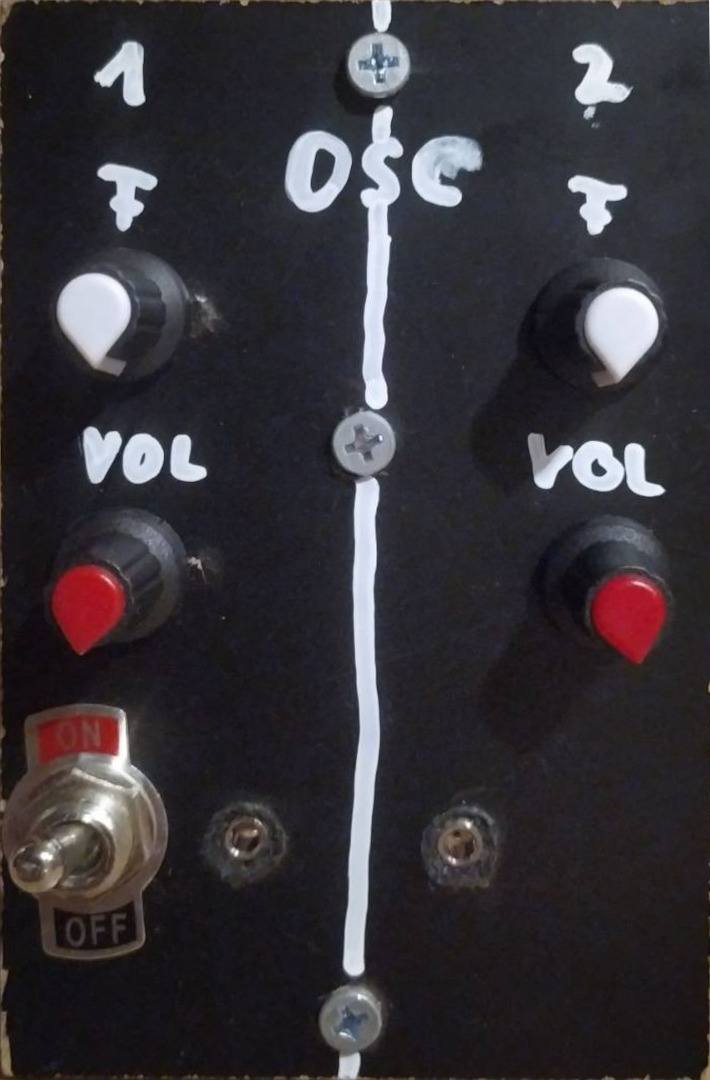
\includegraphics[angle=90,width=.9\linewidth]{/home/felixp/Documents/diplomarbeit/dokumentation/figures/modules/oscillator.jpg}
\caption{\label{fig:org3f2c897}Deckplatte unseres Oszillator-Moduls}
\end{figure}

\begin{figure}
\centering
\begin{circuitikz}[european]
\draw{
(0,0) node[ground, anchor=center, name=G]{}
to[cC, invert, name=C1] ++(0,1)
-- ++(0.5,0)
node[schmitt, anchor=in](S){} (S.out)
-- ++(0,1)
to[pR, l_=R1, name=R1] ++(0,1)
(R1.wiper) -- (R1.wiper -| C1)
-- (C1)

(R1.wiper -| C1)
-- ++(0,1)
-- ++(3,0)
-- ++(0,-2)
-- ++(1,0)

node[op amp, anchor=+](OA1){}
(OA1.out) -- ++(0,1.2)
coordinate (T) -- (T -| OA1.-) -- (OA1.-)

(OA1.out)
to[C, name=C2, l=C2] ++(1,0)
-- ++(0,-0.5)
to[R, name=R2, l=R2] ++(0,-1.5)
node[ground]{}
(C2) -- ++(1,0)

node[op amp, anchor=+](OA2){}
(OA2.out) -- ++(0,1.2)
coordinate (T) -- (T -| OA2.-) -- (OA2.-)

(OA2.out) ++(1,-2.5)
node[ground]{}
to[pR, name=R3, l_=R3] ++(0, 3.5)
-- ++(1,0)
++(0.55,0) node[draw]{OUT}
(R3.wiper) -- (R3.wiper -| OA2.out) -- (OA2.out)
};

\end{circuitikz}
\caption{Schaltkreis einem einzelnen Oszillator, TODO:besser beschreiben \label{fig:schematic_oscillator}}
\end{figure}
\subsection{White Noise \label{Noise}}
\label{sec:org7e196b7}
Noise beziehungsweise Rauschen ist eine Art von Spannungssignal, das auf eine nicht oder schwer vorherzusehende Art und Weise schwingt. Dabei entsteht ein Klang mit einer Vielzahl an Teilfrequenzen. Eine häufige Art von Rauschen ist ""weißes"" Rauschen, bei welchem in einem kleinen Zeitraum alle Frequenzen in einem gegebenen Frequenzspektrum mit annähernd gleicher Amplitude vorhanden sind. Der Name entspringt einer Analogie zu sichtbarem Licht, Beispielsweise deckt weißes Licht alle Frequenzen des sichtbaren Lichtspektrums in gleicher Intensität ab. Eine weitere häufige Art von Rauschen ist rosa Rauschen, bei welchem alle Frequenzen des hörbaren Spektrums abgedeckt werden, jedoch niedrigere Frequenzen in höherer Amplitude vorhanden sind \cite{mt:noise}.

\subsubsection{Spezifikationen}
\label{sec:org744f10d}
Das Noise-Modul stellt weißes Rauschen in einem Bereich \SI{-3}{\volt} bs \SI{3}{\volt} bereit.

\subsubsection{Elektronik}
\label{sec:orgc33b109}
Als Vorlage für das Noise-Modul dient das "`Super simple White Noise Module"' von Kristian Blåsol \cite{miaw:noise}. Dieser Schaltkreis basiert darauf, den Kollektor eines Transistors nicht zu verbinden (siehe Abbildung \ref{fig:schematic_noise} => [n.c]). Dadurch entsteht ein sogenannter Lawineneffekt, welcher üblicherweise ungewünscht ist, in diesem Fall jedoch die Grundlage für unser Rausch-Signal bildet.

\subsubsection{Benutzung}
\label{sec:orgd04cff9}
Weißes Rauschen kann für eine große Anzahl von Zwecken verwendet werden, beispielsweise als \acl{CV} für einen \ac{VCA} oder als Audiosignal. Weißes Rauschen kann dafür benutzt werden, Rauschen anderer "`Farben"' zu erzeugen. Beispielsweise kann rosa Rauschen erzeugt werden, indem dem White Noise Modul ein Tiefpassfilter nachgeschalten wird.

\begin{figure}[htbp]
\centering
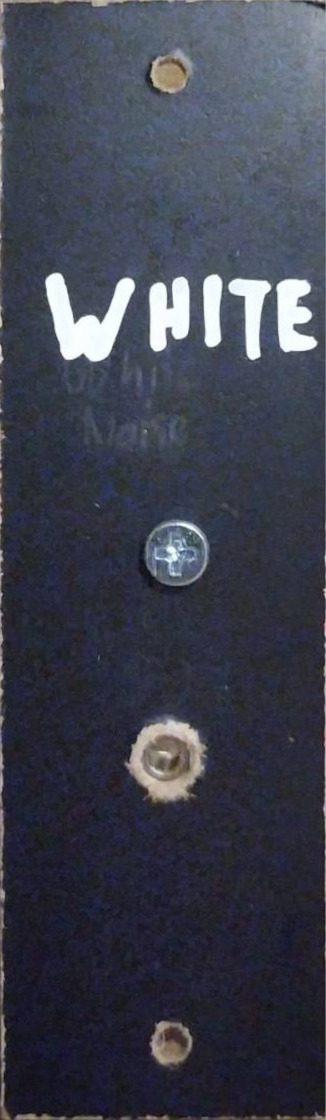
\includegraphics[angle=90,width=.9\linewidth]{/home/felixp/Documents/diplomarbeit/dokumentation/figures/modules/noise.jpg}
\caption{\label{fig:org4f00407}Deckplatte unseres Noise-Moduls}
\end{figure}

\begin{figure}
\centering
\begin{circuitikz}[european]
\draw{
(0,0) node[ground, anchor=center]{} to[R, l=$\SI{470}{\kilo\ohm}$] coordinate (G) ++(0,2) to[C, l=$\SI{47}{\nano\farad}$] ++(3,0) coordinate (B) to[R, l=$\SI{470}{\kilo\ohm}$] ++(2,0) coordinate(A) to[C, l=$\SI{47}{\nano\farad}$] ++(2,0) node[draw,anchor=west]{AUDIO OUT}
(A) to[R, l=$\SI{470}{\kilo\ohm}$] ++(0,2.5) coordinate (T) -- (G|-T) node[npn, rotate=180, xscale=-1, anchor=E, name=Q1]{} ++(0,-2)
(A) -- ++(0,-0.5) node[npn, anchor=C, name=Q2]{} ++(0,-1.5) node[ground, anchor=center]{}
(Q2.B) -- (Q2.B-|B) -- (B)
(Q1.B) -- (Q1.B|-G) -- (G)
(Q1.C) node[draw,anchor=north]{n.c.}
(T) -- ++(0,0.5) node[draw, anchor=south]{\SI{+12}{\volt}}
};
\end{circuitikz}
\caption{Schaltkreis zum Generieren eines Rausch-Signals. \label{fig:schematic_noise}}
\end{figure}
\subsection{Mixer \label{Mixer}}
\label{sec:orgad6147e}
Das Mixer Modul dient dazu, Signale aus mehreren Quellen zu einem einzigen zusammenzuführen. Hierbei kann von jedem Eingang die Lautstärke reguliert werden. Es wird zwischen aktiven und passiven Mixern unterschieden, wobei ein aktiver Mixer die Amplitude der Eingänge nicht nur verkleinern, sondern auch vergrößern kann. Für unseren Synthesizer haben wir uns für eine passive Variante mit drei Eingängen, einem Ausgang und einem invertierenden Ausgang entschieden.

\begin{figure}[htbp]
\centering
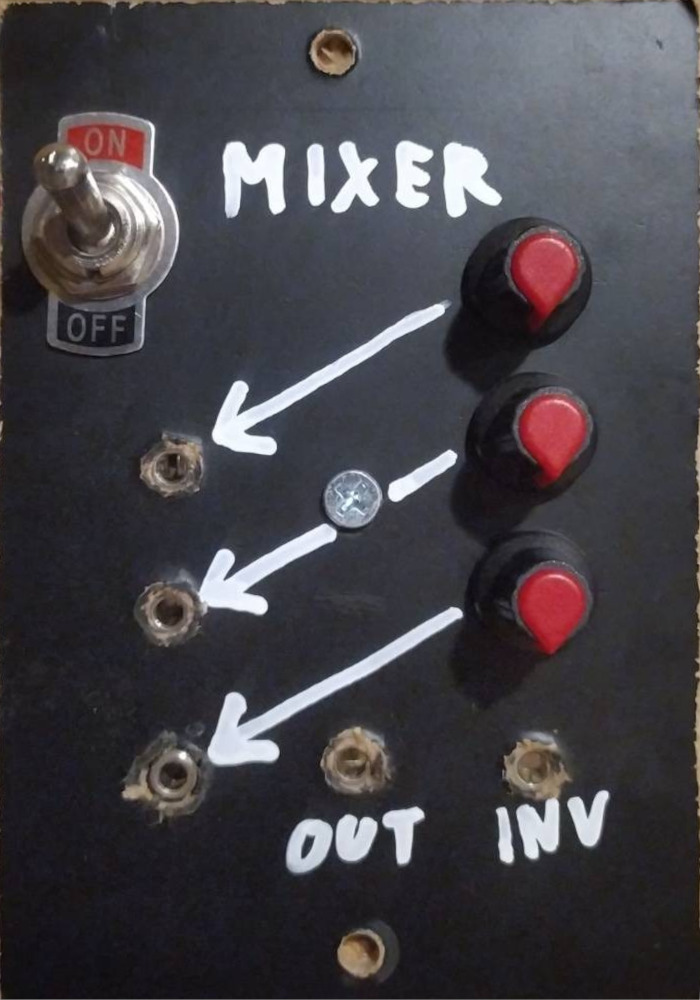
\includegraphics[angle=90,width=.9\linewidth]{/home/felixp/Documents/diplomarbeit/dokumentation/figures/modules/mixer.jpg}
\caption{Deckplatte unseres Mixer-Moduls}
\end{figure}

\subsubsection{Spezifikationen}
\label{sec:org76df691}
Spannung: der volle Spannungsbereich von \SI{\pm12}{\volt} ist sowohl beim Output als auch bei den Inputs möglich.

\subsubsection{Elektronik}
\label{sec:org373afc9}
\cite{miaw:mixer}
\subsubsection{Schematics}
\label{sec:org11470d9}

\begin{figure}[htbp]
\centering
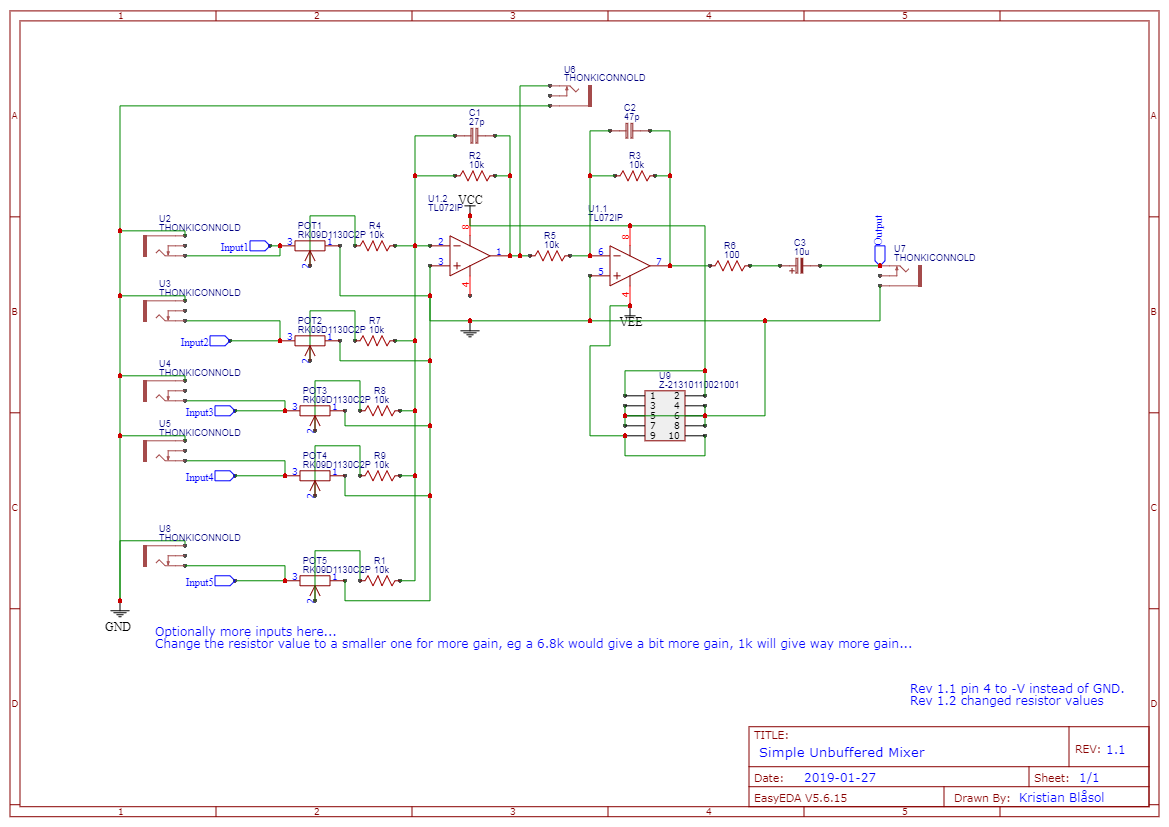
\includegraphics[width=.9\linewidth]{/home/felixp/Documents/diplomarbeit/dokumentation/figures/Schematic_Simple_Mixer.png}
\caption{Schaltkreis für einen passiven Mixer; Quelle: \cite{miaw:mixer}}
\end{figure}
\subsubsection{Benutzung}
\label{sec:orgadc871e}
Es können bis zu drei zu mixende Signale an die oberen Audiobuchsen angeschlossen werden. Die unteren beiden Audiobuchsen liefern das Ausgangssignal, wobei der rechte der invertierende Ausgang ist. Als einfachen Patch könnte man die beiden Signale des Oszillator-Moduls (siehe Abschnitt \ref{Osci}) zusammenführen, um beide Oszillatoren auf einmal zu hören.
\subsection{Spannungskontrollierter Verstärker \label{VCA}}
\label{sec:org6227b08}
Ein \acf{VCA} verstärkt ein angelegtes Signal um einen Faktor, welcher proportional zur angelegten \acl{CV} ist. \acp{VCA} sind essentiell, um den erzeugten Klängen einen Rhythmus zu verleihen, da ohne \ac{VCA} keine dynamische Lautstärkeänderung möglich ist. 
\subsubsection{Spezifikationen}
\label{sec:orge26fc09}
\subsubsection{Elektronik}
\label{sec:orgdbe75c0}
Es gibt eine Vielzahl von möglichen Ansätzen für die technische Umsetzung eines \ac{VCA}. Die simpelste Möglichkeit ist es wohl, eine Vactrol zu benutzen, da diese mit nur minimaler Beschaltung zu einem VCA umgewandelt werden kann todo: schematic einfügen:\url{https://www.dropbox.com/s/o6oiyanco8lzmvt/Schematic\_Vactrol.pdf?dl=0}. Jede Art von \ac{VCA} hat einen gewissen Eigenklang, wobei ein Vactrol-VCA eine sehr "`glatte"' Dynamik erzeugt. Abrupte Spannungsänderungen in der \acl{CV} werden geglättet, wodurch das ausgehende Signal nur eine stetige Änderung in der Lautstärke erfahren kann.

Ein weiterer Ansatz nutzt den linearen Reaktionsbereich zweier NPN-Transistoren, wobei durch die Beschaltung auf einem der Transistoren genau das gegenteilige Signal, allerdings mit dem gleichen positiven Offset erzeugt wird. Diese zwei Signale werden dann von einem Operationsverstärker voneinander abgezogen, wodurch der positive Offset eliminiert wird und das modulierte Signal übrig bleibt. Eine Vielzahl von selbstregelnden Rückkopplungsschleifen trägt dazu bei, dass diese Art von \ac{VCA} besonders stabil und schnell auf Änderungen in der angelegten Kontrollspannung reagieren kann.
\subsubsection{Schematics}
\label{sec:org1b39f69}
\subsubsection{Benutzung}
\label{sec:org1f3461d}
\acp{VCA} können durch eine Vielzahl an Modulen angesteuert werden. Am häufigsten ist wohl eine Art von Hüllkurvengenerator, um die Lautstärkeänderung bei einem Tastenanschlag zu simulieren. Ein einfacheres Beispiel wäre eine Rechteckswelle von einem LFO, um eine Art Stakkato zu erzeugen, oder ein langsam schwingender Sinus für eine Art Wobbel-Effekt.
\subsection{Low Frequency Oscillator \label{LFO}}
\label{sec:orgad8da16}

Ein \ac{LFO} generiert ein Signal, welches in einem niedrigen Frequenzbereich oszilliert. Wir benutzen als Vorlage für unseren \ac{LFO} den "`Simple LFO"' von David Haillant \cite{haillant:lfo}. Dieses Modul erzeugt langsam oszillierende Spannungen in Form einer Rechteckwelle und einer Dreieckwelle.

\begin{figure}[htbp]
\centering
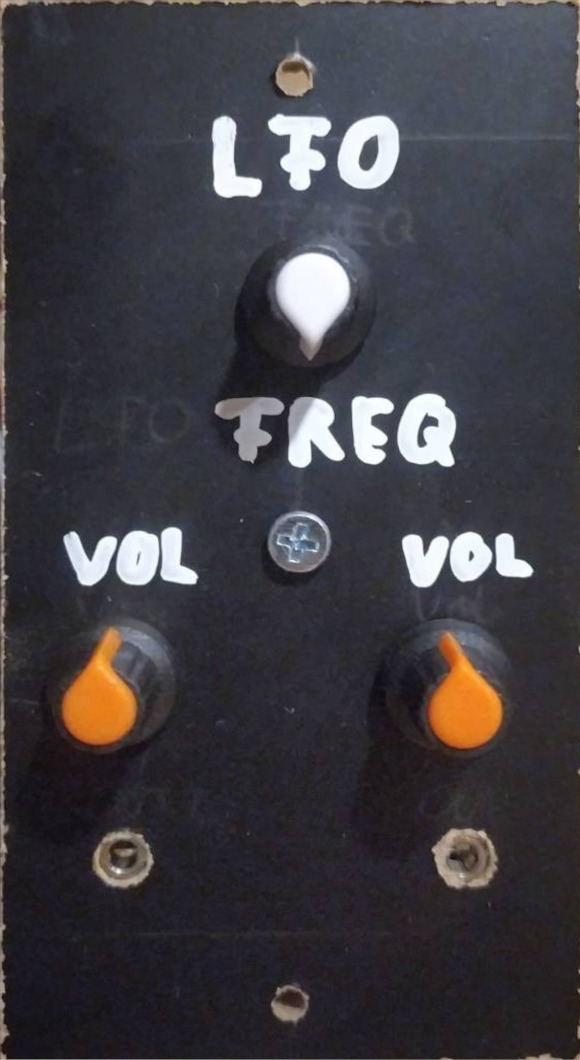
\includegraphics[width=.9\linewidth]{/home/felixp/Documents/diplomarbeit/dokumentation/figures/modules/LFO.jpg}
\caption{Deckplatte unseres LFO-Moduls}
\end{figure}


\subsubsection{Spezifikationen}
\label{sec:org812a5e2}
Typische Oszillationsbereiche für \acp{LFO} liegen bei \SI{0.1}{\hertz} bis \SI{10}{\hertz}. Das  von uns gewählte Design erzeugt jeweils einen Rechteck- und Dreiecksausgang. Da beide Signale aus dem selben Schwingkreis stammen, kann die Frequenz nicht unabhängig geändert werden, die Amplituden der beiden Signale sind jedoch individuell einstellbar.

\subsubsection{Elektronik}
\label{sec:org08d19c6}
Wir verzichten bei unserer Ausführung des Moduls auf die vorgesehene Leuchtdiode, welche einen visuellen Indikator für die Frequenz des Ausgangssignals bieten würde. Dadurch wird am verwendeten TL074 ein Operationsverstärker frei. Dieser wird als zweiter Puffer benutzt, um beide Wellenformen parallel ausgeben zu können. Die Frequenz beider Wellenformen ist gekoppelt und wird über ein einzelnes Potentiometer gesteuert, die Amplituden sind separat anzusteuern.

\subsubsection{Schematics}
\label{sec:org5598e56}

\subsubsection{Benutzung}
\label{sec:org097cfa5}
\acp{LFO} können für viele verschiedene Zwecke genutzt werden, der simpelste davon ist, das erzeugte Signal direkt als Audio auszugeben. Häufiger wird die Spannung eines \acp{LFO}s als \acl{CV} genutzt, beispielsweise als Trigger für einen Hüllkurvengenerator oder zum Ansteuern eines \acp{VCA}, um eine Funktion ähnlich eines Arpeggiators zu erfüllen.

Der mittig oben platzierte Drehknopf steuert die Frequenz der beiden Signale, die zwei Drehknöpfe und Buchsen dienen zur Lautstärkeregelung und Signalausgabe.
\subsection{Attack-Release Hüllkurvengenerator \label{AR}}
\label{sec:org150c8ee}
Hüllkurvengeneratoren sind Module, welche bei Eingang eines Gate-Signals eine Hüllkurve generieren. Diese kann beispielsweise dazu genutzt werden, einen \ac{VCA} anzusteuern, welcher einem Klang Rhythmus und Dynamik, also eine sich Ändernde Lautstärke verleiht. Aufgrund der Komplexität eines vollständigen \ac{ADSR} Hüllkurvengenerators haben wir uns dazu entschieden, einen simpleren \ac{AR} Hüllkurvengenerator zu bauen. Dieser besitzt einen Eingang für eine \acl{CV}, an welchen ein Gate-Signal angelegt werden kann und zwei Drehpotentiometer, mit denen die Parameter Attack und Release eingestellt werden können. Attack stellt dabei die Zeit dar, die das Signal nach dem Drücken einer Taste beziehungsweise nach dem Anfang eines eingehenden Gate-Signals benötigt, um seinen Maximalwert zu erreichen. Release stellt die Zeit dar, die die Spannung der Hüllkurve nach dem Schließen des Gates benötigt, um wieder \SI{0}{\volt} zu erreichen.

\begin{figure}[htbp]
\centering
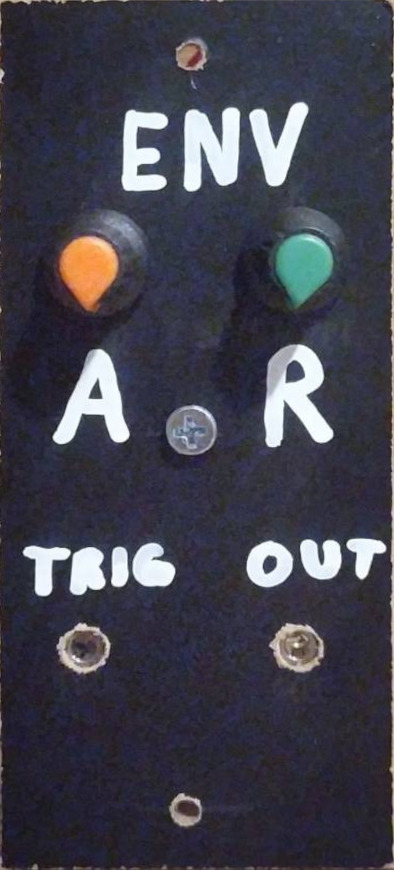
\includegraphics[width=.9\linewidth]{/home/felixp/Documents/diplomarbeit/dokumentation/figures/modules/AR.jpg}
\caption{Deckplatte unseres AR-Hüllkurvengenerator-Moduls}
\end{figure}

\subsubsection{Spezifikationen}
\label{sec:org8d4fbc8}
\subsubsection{Elektronik}
\label{sec:org0b2b8be}
In unserer Umsetzung wird das Potential am Eingang für eine \acl{CV}, an welchem ein Gate-Signal erwartet wird, von einem Operationsverstärker auf 12V verstärkt. Durch den oberen Signalpfad füllt sich ein großer Kondensator. Die Spannung, welche am Kondensator anliegt, wird gleichzeitig von einem Spannungsfolger gepuffert, da diese auch die Ausgangsspannung darstellt. Wird das Gate geschlossen, fällt die Spannung über den unteren Signalpfad wieder ab. Durch die Potentiometer kann man die Geschwindigkeit dieser beiden Prozesse kontrollieren.
\subsubsection{Schematics}
\label{sec:orgfa448c3}
\begin{figure}[htbp]
\centering
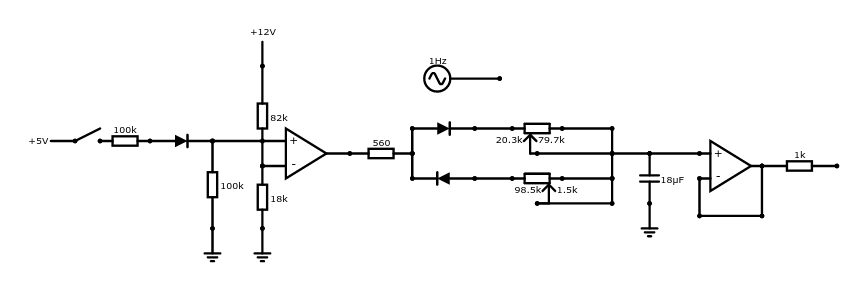
\includegraphics[width=.9\linewidth]{/home/felixp/Documents/diplomarbeit/dokumentation/figures/Schematic_AR.png}
\caption{Schaltkreis für einen simplen Attack Release Hüllkurvengenerator; Quelle: \cite{synthnerd:ar}}
\end{figure}
\subsubsection{Benutzung}
\label{sec:org1c84ed6}
Unser AR bietet einen Eingang für Kontrollspannung vom Typ Gate, welcher angibt, ob etwa eine Taste gedrückt oder nicht. Außerdem ist ein Ausgang für die Hüllkurve vorhanden, welcher als \acl{CV} für einen \ac{VCA} vorhergesehen ist.
